% ВАЖНО
% Не меняйте ничего в этом файле. А если меняете, то делайте это в этом проекте:
% https://github.com/kib-courses/latex_templates
% Для пользовательских настроек есть файл ./header/user.tex
\documentclass{beamer}
\usetheme{metropolis} 
\usecolortheme{rose}

\hypersetup{unicode=true}
\usepackage{tikz}

\usepackage{xcolor}
\usepackage[utf8]{inputenc}
\usepackage{hyphenat}
\usepackage[russian,english]{babel}          % Use metropolis theme
\usepackage{wrapfig}

\usepackage[normalem]{ulem}  % для зачекивания текста

\usepackage{caption}
\captionsetup[figure]{name=Рисунок }
\newcommand{\рис}[1]{рис.\ref{#1}}
\newcommand{\Рис}[1]{Рис.\ref{#1}}


\captionsetup[table]{name=Таблица~№}
\newcommand{\таблицa}[1]{таблица~№\ref{#1}} % именительный падеж
\newcommand{\таблицы}[1]{таблицы~№\ref{#1}} % родительный падеж
\newcommand{\таблице}[1]{таблице~№\ref{#1}} % дательный и предложный падеж
\newcommand{\таблицу}[1]{таблицу~№\ref{#1}} % винительный падеж
\newcommand{\таблицей}[1]{таблицей~№\ref{#1}} % творительный падеж 
\newcommand{\Таблицa}[1]{Таблица~№\ref{#1}} % именительный падеж
\newcommand{\Таблицы}[1]{Таблицы~№\ref{#1}} % родительный падеж
\newcommand{\Таблице}[1]{Таблице~№\ref{#1}} % дательный и предложный падеж
\newcommand{\Таблицу}[1]{Таблицу~№\ref{#1}} % винительный падеж
\newcommand{\Таблицей}[1]{Таблицей~№\ref{#1}} % творительный падеж 

\setbeamertemplate{footline}[frame number] % указывает на каждой странице общее количество страниц

% Указывайте все новые термины в \termdef команде. А уже известные ранее или из других курсов в \term
\newcommand{\termdef}[1]{\textbf{\textit{#1}}}
\newcommand{\term}{\textit}

% Диалог с аудиторией.
\newcommand{\auditorium}[1]{\textcolor{red}{\textbf{#1}}}

\let\OLDhref\href
\renewcommand{\href}[2]{\textcolor{blue}{\OLDhref{#1}{#2}}}

% \setbeameroption{show notes}
% \usepackage{listings}             % Include the listings-package
% \usepackage{minted}

\usepackage{CJKutf8}

\title{Лекция 1. Экспертные системы, полнота, точность. Задачи ИБ, решаемые ЭС.}
% \date{\today}
\date{17 сентября 2019}
\author{Павел Владимирович Слипенчук}
\institute{Москва, МГТУ им.Бауманка,\\ каф.ИУ-8, \href{https://t.me/kibinfo}{КИБ}}
% \titlegraphic{\includegraphics[width=2cm]{logo_ur.jpg}}
\titlegraphic{\small \href{https://github.com/kib-courses/dsis}{Data Science для решения задач информационной безопасности}}

\begin{document}
  \maketitle
    
  \begin{frame}{План лекции}
    \begin{enumerate}
    \item \nameref{section:history_remarks}
    \item \nameref{section:expert_systems_recall_presision}
    \item \nameref{section:is_tasks}
	\end{enumerate}
 \end{frame}
 
 \section{История. Заметки}\label{section:history_remarks}
  
  \begin{frame}{Гомеоскоп Корсáкова}
    \textbf{Семён Павлович Корсáков}
    (1787-1853) 
    -- изобретатель первых экспертных систем 
    (механических): гомеоскопов, применявшихся в медицине.  
    \begin{center}
    		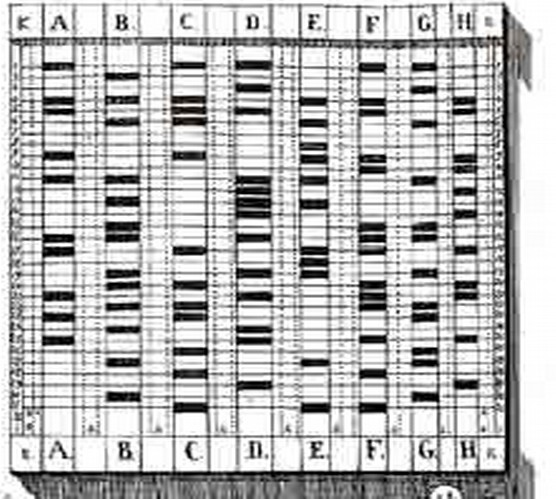
\includegraphics[width=4.5cm]{../pic/gomeoskop.png}\centering
    		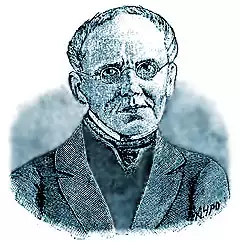
\includegraphics[width=4cm]{../pic/korsakov.png}\centering
    \end{center}
    Домашнее задание: \url{https://ru.wikipedia.org/wiki/Гомеоскоп}
  \end{frame}
  
  \begin{frame}{XVII-XIX}
     \begin{itemize}
        \item \textbf{
         \href{https://ru.wikipedia.org/wiki/\%D0\%A1\%D1\%83\%D0\%BC\%D0\%BC\%D0\%B8\%D1\%80\%D1\%83\%D1\%8E\%D1\%89\%D0\%B0\%D1\%8F_\%D0\%BC\%D0\%B0\%D1\%88\%D0\%B8\%D0\%BD\%D0\%B0_\%D0\%9F\%D0\%B0\%D1\%81\%D0\%BA\%D0\%B0\%D0\%BB\%D1\%8F}{<<Паскалина>>}}  -- суммирующая машина Блеза Паскаля (1642).
        \item Разностная машина Иоганна Мюллера (1788, не построена)
        \item Разностная машина Чарльзя Бебиджа (малая 1822, построена; большая 1849, построена в 2000)
        \item Гомеоскоп С.Н.Корсакова (1832) 
     \end{itemize}
  \end{frame}
 
   \begin{frame}{1930-е}
     \begin{itemize}
     	\item Советский физиолог 
     	Пётр Кузьмич Анохин
     	формулирует понятие <<обратной связи>> (1935)
 	    \item Взлом шифровальной машины <<Энигма>> (Мариан Реевски).
 	    Проект <<Бомба>> (Ежи Рожицки, Генрих Зыгальски).
 	    Передача чертежей и спецов в Кабацком лесу под Варшавой 
 	    английской разведке (1936).
 	    Проект <<Колосс>> (под руководством Алана Тьюринга,1936-1941)
 	    \item Фашистский антикварный проект (первый гипертекст, 1937)
 	    \item Первые ЭС для военных целей (зенитные орудия, ТАУ, 1939).
 	    \item Системы автоматического регулирования (САР),
 	    Владимира Викторовича Солодовникова (1939)
      \end{itemize}
   \end{frame}

     \begin{frame}{1940-е}
   \begin{itemize}
   	\item Машина Конрада Цузе (1941) 
   	и высокоуровневый язык програмирования: Планкалкюль (1948)
   	\item ENIAC Джона Мокли
   	и
   	Джона Преспера Эккерта
   	(1943, 1946 публично представлен)
   	\item ~<<Кибернетика>>
   	Норберта Винера (1948)
   \end{itemize}
\end{frame}

   \begin{frame}{В.М.Глушков \& А.И.Китов. Проект ОГАС.}
	  \begin{itemize}
	  	\item ОГАС\footnote{Общегосударственная Автоматизированная Система}
	  	и ЕГСВЦ\footnote{Единая Государственная Сеть Вычислительных Центров}
	  	Анатолия Ивановича Китова
	  	и
	  	Виктора Михайловича Глушкова.
	  	(1958-1964).
	  	\item МИР\footnote{Машина для инженерных расчётов} Глушкова -- первый ПК.
	  \end{itemize}
     (!) В 1964 году выходит статья в The Washington Post <<Перфокарта управляет Кремлём>>,
     после которой Политбюро ЦК КПСС принимает решение о сворачивании проекта ОГАС. 
     
     \auditorium{ДЗ. Проект <<Киберсин>> в Чили.}
	\end{frame}
  
  \begin{frame}{Машинное обучение. Пионеры}
    \begin{itemize}
  	  \item Метод опорных векторов
  	  (Support vector machine)
  	  Алексея Яковлевича Червоненкиса
  	  и
  	  Владимира Наумовича Вапника (1963). 
  	  \item Случайный лес
  	  (Random Forest)
  	  Юрия Леонидовича Павлова (1977)
  	  \item Bootstrap 
  	  Бредли Эйфон (1977)
  	  \item Байесовские сети
  	  Джуды Перла
  	  Judea Pearl
  	  (1988)
  	  \item Bagging
  	  (Bootstrap Aggregating)
  	  Лео Бреймана
  	  (1994)
  	  \item Boosting
  	  Роберта Шапира 
  	  (1990)
    \end{itemize}
  \end{frame}

 
 
 \begin{frame}{Машинное обучение. Пионеры}
 \begin{itemize}
 	\item “Закон Мура” и появление
 	доступных
 	персональных компьютеров
 	открыло новую эпоху в ML и DM  
 	(1990 – н.в.)
 	\item первая\footnote{после появления релационной алгебры}
 	NoSQL СУБД
 	“Strozzi NoSQL”
 	Карло Стрози
 	(1998) 
 \end{itemize}
\end{frame}

  \section{Экспертная система. Априорная и апостериорная вероятности. Полнота, точность экспертной системы.}\label{section:expert_systems_recall_presision}
  
  \begin{frame}{Экспертная система}
   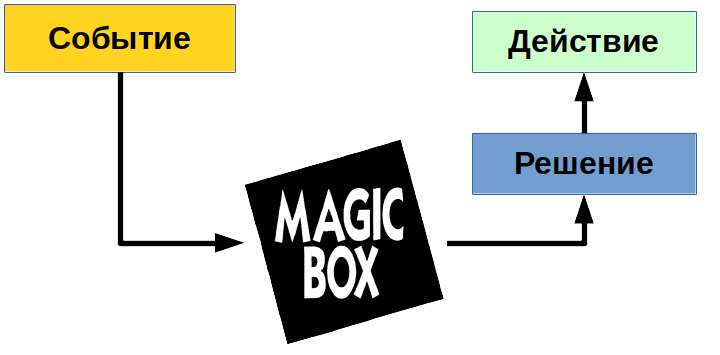
\includegraphics[width=10cm]{../pic/expert_system_1.png}
  
  Процесс:
  \begin{enumerate}
  	\item Событие
  	\item Экспертная система
  	\item Решение (экспертной системы)
  	\item Действие (основанное решением экспертной системы)
  \end{enumerate}
  \end{frame}

  \begin{frame}{ФМ система RSA}
   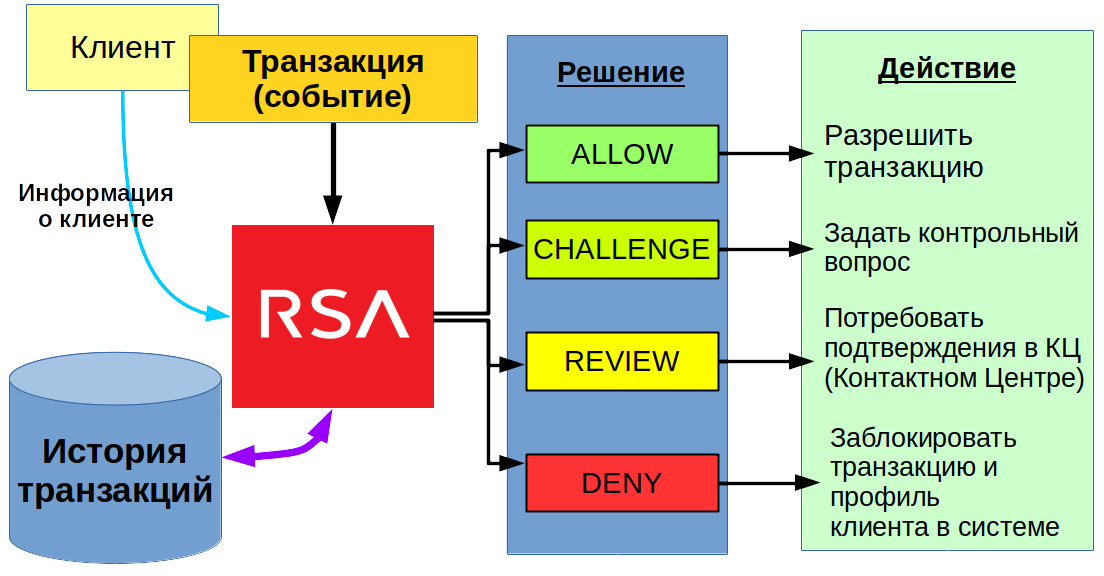
\includegraphics[width=11cm]{../pic/expert_system_rsa.png}
  
  Есть открытое описание бизнес-процессов в Хакере:
  \url{https://xakep.ru/2017/05/22/bank-antifraud-uncovered/}
  \end{frame}
  
  \begin{frame}
  	\begin{block}{Замечание.}
  		Для улучшения качества работы экспертной системы, понимания границ ее применения,
  		необходимо знать о её внутреннем устройстве.
  		
  		Но для оценки её качества на тестовых данных, ЭС можно воспринимать как чёрный ящик.
  		Таким образом, чтобы принять работу, не требуется быть специалистом в области DS/ML.
  	\end{block}
  \end{frame}

  \begin{frame}{Априорная и апостериорная вероятности}
  
  \termdef{Априорная вероятность} -- вероятность взятая из каких-либо умозаключений или правил.
  Примеры:
  \begin{enumerate}
  	\item Вероятность выпадения орла 0.5, потому что он ничем не лучше и не хуже решки и монетка не может упасть ребром (это пренебрежимо мало)
  	\item Мы отправили \term{событие} на вход ЭС и получили на выходе решение: "вероятность мошенничества равна 0.7 для данного события".
  \end{enumerate}
   
  \end{frame}

  \begin{frame}{Априорная и апостериорная вероятности}
  	\small
\termdef{Апостериорная вероятность} -- статистическая вероятность\footnote{
	Вообще то говоря, апостериорная вероятность имеет более глубокий и широкий смысл.
	Но в рамках нашего курса апостериорная вероятность -- это просто статистическая доля того или иного события.}, посчитанная на каких-либо конкретных данных.

	Примеры: \small
	\begin{enumerate}
		\item Мы 100 раз подбросили монету и 47 раз выпал орёл. Следовательно 
		вероятность выпадения орла 0.47
		\item Мы взяли экспертную систему и посчитали, что "вероятность мошенничества 0.7"
		выпало на 67 мошеннических и 34 легитимных операций за определённое время. 
		Значит \term{точность} системы для данного \term{решения} на данном промежутке времени равна $\frac{67}{67+34} \approx 0.66$; что примерно равно $0.7$ -- следовательно систему можно считать адекватной.
	\end{enumerate}
\end{frame}
  
  \begin{frame}
  Современные ЭС состоят из двух блоков:
  \begin{enumerate}
  	\item \termdef{Score Engine} -- программный модуль, выдающий значение скоринга (как правило от 0 до 1000, от 0.0 до 1.0 или от -1.0 до 1.0). Чем выше это значение, тем больше
  	\textit{априорная вероятность} что произошёл какой-либо инцидент.
  	Score Engine выдает либо одно значение (\href{https://www.rsa.com/en-us/products/fraud-prevention}{RSA}) 
  	либо несколько (\href{https://www.group-ib.ru/secure-bank.html}{Secure Bank}, Group-IB).
  	\item \termdef{Rules Engine} -- программный модуль, использующий данные Score Engine и другие данные 
  	и выдающий \term{решение} экспертной системы.
  \end{enumerate}

  Иногда ЭС называют только Score Engine. Таким образом получаем большое разнообразие решений вида: "априорная вероятность мошенничества равна X".
  \end{frame}
  
   \begin{frame}{Экспертная система}
       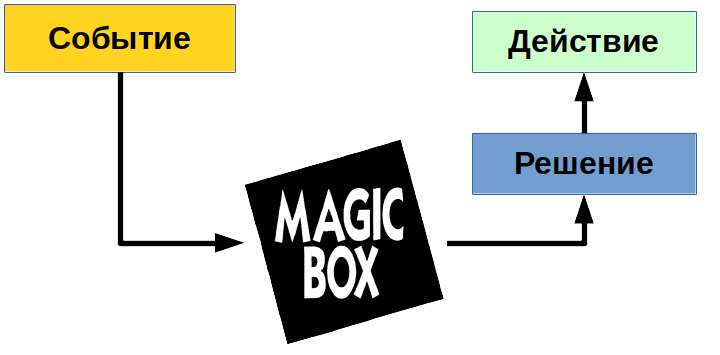
\includegraphics[width=10cm]{../pic/expert_system_1.png}
       
       Как понять, как хорошо работает экспертная система?
   \end{frame}
  
  \begin{frame}{Ложная сработка \& пропуск цели} 
  \centering
  \LARGE
  \begin{tabular}{l|l}
  	Ошибка I рода & Ошибка II рода \\
  	$\alpha$ ошибка & $\beta$ ошибка \\
  	false positive (fp) & false negative (fn) \\ 
  	Ложная сработка  & Пропуск цели \\
  \end{tabular}
  \end{frame}

  \begin{frame}{Четыре события}
  \small На примере задачи фрод-мониторинга в банковской сфере.
  \begin{enumerate}
  	\item $F_r$ (fraud real) -- событие, означающее что банковская операция в действительности является мошеннической. 
  	\item $F_s$ (fraud system) -- событие, когда некая система фрод-мониторинга оценила данную операцию как мошеннической.
  	\item $L_r$ (legitim real) -- событие, означающее что банковская операция в действительности является легитимной (не мошеннической).
  	\item $L_s$ (legitim system) -- событие когда некая система фрод-мониторинга оценила данную операцию как легитимную (не мошеннической).
  \end{enumerate}
  События $F_s$ и $L_s$ \term{несовместны}, 
  а так же $F_r$ и $L_r$ \term{несовместны}.
  \end{frame}

  \begin{frame}
  Таким образом можно рассматривать следующие события: 
  $P(F_r \cap F_s)$, $P(F_r \cap L_s)$, $P(L_r \cap F_s)$, $P(L_r \cap L_s)$. 
  Для удобства будем обозначать их просто: 
  $P(F_r  F_s)$, $P(F_r L_s)$, $P(L_r F_s)$, $P(L_r L_s)$. 
  
  Так же имеет смысл рассматривать условные вероятности: 
  $P(F_r | L_s)$,
  $P(F_s | L_r)$,
  $P(F_r | F_s)$, 
  $P(F_s | F_r)$, ... .
  \end{frame}

  \begin{frame}{Ложная сработка \& пропуск цели} 
  \begin{center}
		\LARGE
		\begin{tabular}{l|l}
		 	Ошибка I рода & Ошибка II рода \\
		 	$\alpha$ ошибка & $\beta$ ошибка \\
		 	false positive (fp) & false negative (fn) \\ 
		 	Ложная сработка  & Пропуск цели \\
		 	$P(L_r|F_s)$ & $P(F_r |L_s)$\\
		\end{tabular}
  \end{center}
   
    \begin{block}{Замечание.}
 	Иногда false positive называют событие $P(L_r F_s)$, а не $P(L_r | F_s)$.
 	Аналогично false negative называют $P(F_r  L_s)$, а не $P(F_r | L_s)$.
 	Это очень важно! Не запутайтесь!
    \end{block}
  \end{frame}
 
  \begin{frame}{Полнота \& точность}\label{frame:presicion_recall}
  Основными показателями качества системы являются 
  \termdef{полнота} ($\Pi$, \termdef{recall}) 
  и 
  \termdef{точность} ($T$, \termdef{precision}).
  
  Их определения:
  \begin{equation}
  \Pi \stackrel{def}{=} P(F_s | F_r)
  \end{equation}
  \begin{equation}
  T \stackrel{def}{=} P(F_r | F_s)
  \end{equation}
  
  Полноту и точность можно вычислить через формулы:
  \begin{equation}\label{eq:recall_calc}
  \Pi = \frac{P(F_s  F_r)}{P(F_s F_r) + P(L_s F_r)}
  \end{equation}
  \begin{equation}\label{eq:precision_calc}
  T = \frac{P(F_s F_r)}{P(F_s F_r) + P(F_s L_r)}
  \end{equation}
  \auditorium{ДЗ: докажите эти формулы.}
  
  \auditorium{ДЗ: посмотрите  \href{https://en.wikipedia.org/wiki/Precision_and_recall}{определения в англоязычной Википедии} $T$ и $\Pi$.}
  \end{frame}
  
  \begin{frame}{Использование формул \eqref{eq:recall_calc} и \eqref{eq:precision_calc}}\label{frame:precision_calc_example}
  \small
  Формулы \eqref{eq:recall_calc} и \eqref{eq:precision_calc} полезны 
  для определения полноты и точности через статистические данные.
  
  Предположим, что в каком-либо банке за определенный промежуток времени
  произошло \textbf{562} мошеннических транзакций. 
  Выберем их все и случайным способом ещё \textbf{100 000} легитимных транзакций.
  Предположим что всего за этот промежуток произошло 67 234 134 234 операций. 
  
  Тогда наша выборка легитимных операций это $1/q$ от общей доли, где: 
  \begin{equation*}
  q = \frac{67234134234}{100000} \approx 672 \cdot 10^3
  \end{equation*}
  
  Мы прогнали все эти транзакции через ЭС и обнаружили количество пар событий:
  $C(F_s F_r)= 386$, 
  $C(F_s L_r)= 18$, 
  $C(L_s F_r)= 176$, 
  $C(L_s L_r)= 999 982$.
   
  ... ... ... ...
  \end{frame}
   
  \begin{frame}{Использование формул \eqref{eq:recall_calc} и \eqref{eq:precision_calc}} 
  ... ... ... ...
  
  Таким образом через формулу  \eqref{eq:precision_calc} можно найти точность:
  \begin{eqnarray*}
  T = \frac{P(F_s F_r)}{P(F_s F_r) + P(F_s L_r )} = 
  \frac{C(F_s F_r)}{C(F_s F_r) + q \cdot C(F_s L_r)}  = \\
  \approx \frac{386}{386 + 18 \cdot  672 \cdot 10^3 }
  \approx \frac{386}{18 \cdot  672 \cdot 10^3 }
  \approx 3 \cdot 10^{-5}
  \end{eqnarray*}
  
  \begin{block}{Замечание}
  	Очень часто при подсчёте точности забывают про коэффициент $q$ 
  	и совершают ошибку, измеряя точность на конкретных данных.
  	На практике физически невозможно выбрать все легитимные транзакции,
  	поэтому берут их подмножество.
  \end{block}

  \auditorium{ДЗ: найдите полноту. Зависит ти она от $q$?}
  \end{frame}
  
  \begin{frame}{$O_1$ и $O_2$ через $\Pi$ и $T$}
  Ошибки I и II рода можно выразить через полноту и точность.
  
  \begin{equation}\label{eq:O_2_from_recall}
  O_2 = 1 - \Pi
  \end{equation}
  
  \begin{equation}\label{eq:O_1_from_recall_and_presicion}
  O_1 = \frac{P(F_r)}{P(L_r)} \cdot \Pi \cdot \left( \frac{1}{T} - 1 \right)
  \end{equation}
  
  \auditorium{ДЗ. Докажите формулы 
  \eqref{eq:O_2_from_recall}
  и
  \eqref{eq:O_1_from_recall_and_presicion}
  }
  
  \auditorium{ДЗ. Выразите полноту и точность, через $O_1$ и $O_2$}
  \end{frame}
  
  \begin{frame}
  \LARGE
  \centering
  Пропуск цели
  
  vs
  
  Ложная сработка
  
  \auditorium{Что важнее?}
  \end{frame}

  \begin{frame}
  ЭС диагностики раковой опухоли:
  \begin{itemize}
    \item \textbf{Ложная сработка} -- 
    решение ЭС в том, что пациент болен; но на самом деле пациент здоров.
    \item \textbf{Пропуск цели}
    -- система говорит больному раком пациенту, что он здоров.
  \end{itemize}
  
  ЭС обнаружения превышения скорости автомобиля:
  \begin{itemize}
    \item \textbf{Ложная сработка}
    -- штраф будет выписан добропорядочному водителю.
    \item \textbf{Пропуск цели}
    -- лихач не будет наказан за превышение скорости и ему не выпишут штраф
  \end{itemize}
  \end{frame}
  
  \begin{frame}{Сложные случаи}
  Фрод мониторинг
  \begin{itemize}
  	\item \textbf{Ложная сработка}
  	-- заблокировать легитимную транзакцию.
  	\item \textbf{Пропуск цели}
  	-- позволить хакерам украсть деньги клиента
  \end{itemize}
  
  На практике: определяют допустимое количество нагрузки на контактный центр и 
  забивают эту нагрузку <<под завязку>>.
  
  Отсюда выводы: мелкие хищения менее интересны чем крупные.
  \end{frame}

  \begin{frame}{Булев(ый) и вероятностный отклик}
  \small
  \termdef{Булев(ый) отклик} -- либо 0, либо 1. Либо -1, либо 1. (виновен/не виновен).
  
  \termdef{Вероятностный отклик} -- классификатор выдает вероятностное 
  \term{априорное} решение $p \in [0, 1]$:
  0 -- нет, 1 -- да, 0.5 -- неопределенно.
  (или $p \in [-1, 1]$: $-1$ --нет, $0$ -- не определено, $1$ -- да.)
  
  Любое вероятностное решение можно свести к булевому.
  Для этого определяется некое значение, называемое
  \termdef{отсечкой} (cutoff, offset):
  \begin{equation}
  p \geqslant cutoff \Longrightarrow return ~ 1
  \end{equation}
  \begin{equation*}
  p < cutoff \Longrightarrow return ~ 0
  \end{equation*}
  
  \begin{block}{Замечание}
  Значения $p$ -- это \term{априорные вероятности} ЭС.
  Они могут не иметь никакого отношения к реальности
  \end{block}
  \end{frame}

  \begin{frame}{Влияние отсечки на полноту и точность}
  Было: 
  \begin{center}
   $p \geqslant 0.5$ – виновен; $р<0.5$ – не виновен
\end{center}
  Поменяли отсечку. Стало:
  \begin{center}
     $p \geqslant 0.8$ – виновен; $р<0.8$ – не виновен
  \end{center}
   
   \auditorium{
  Что стало с полнотой и точностью? Что стало с ложной сработкой 
  и пропуском цели? Что не увеличилось, а что не уменьшилось?}
  \end{frame}

  \begin{frame}{ROC-кривая}\label{frame:roc}
  \centering
   Receiver Operating Characteristic
   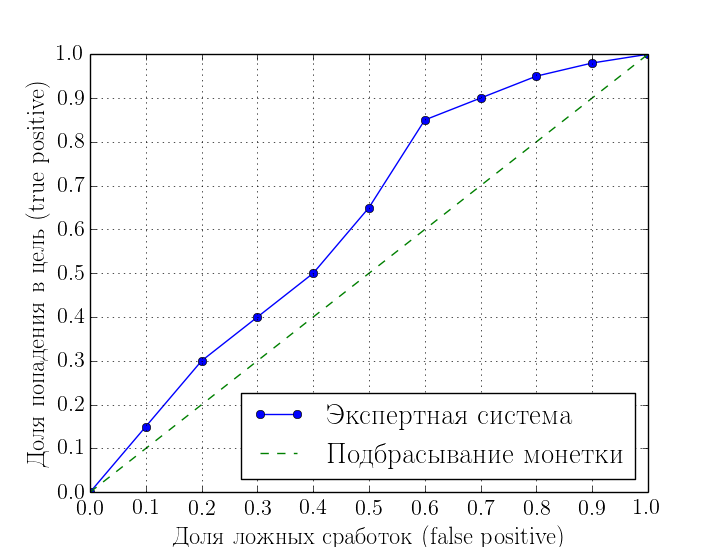
\includegraphics[width=10cm]{../pic/roc_example.png}
   \end{frame}

  \begin{frame}{Коэффициент Джини \& Максимальное отклонение (<<Расстояние Робина Гуда>>)}
   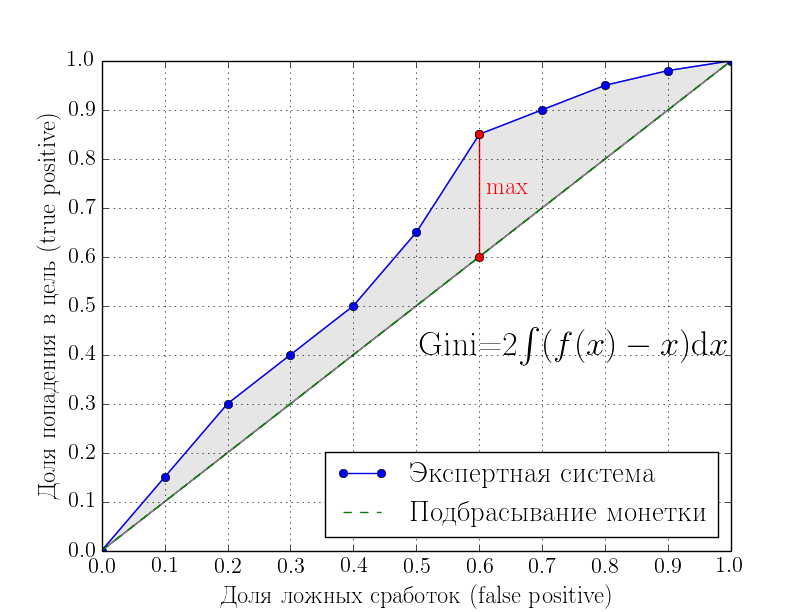
\includegraphics[width=10cm]{../pic/gini_coef.png}
  \end{frame}

  \begin{frame}{Используемые области}
	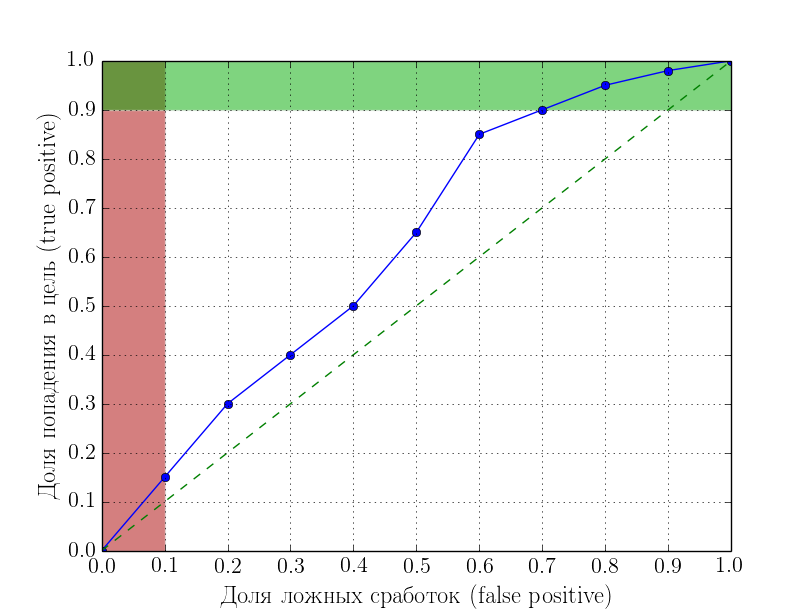
\includegraphics[width=9cm]{../pic/roc_example_2.png}
   \small
   
	Какие области используются для детектирования рака 
	и для обнаружения превышения скорости
	автомобилей?
   \end{frame}


  \begin{frame}{А эти области никогда не используются???}
	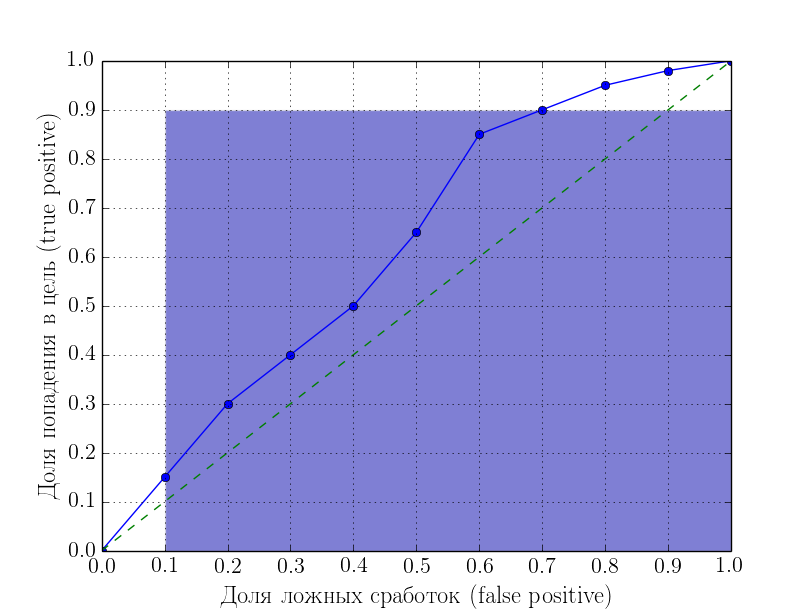
\includegraphics[width=11cm]{../pic/roc_example_3.png}

  \end{frame}

  \begin{frame}{Ансамбли}
  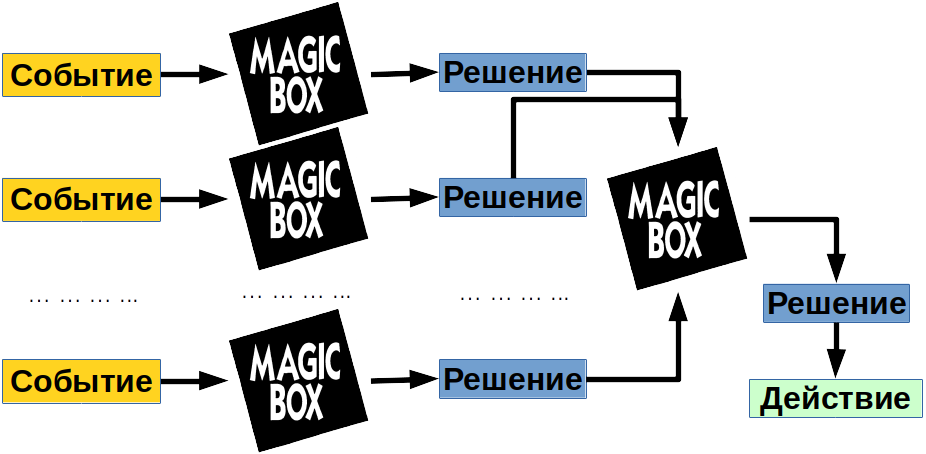
\includegraphics[width=11cm]{../pic/ensemble_example.png}
  \end{frame}

  \section{Задачи ИБ, решаемые экспертными системами}\label{section:is_tasks}
	
  \begin{frame}{Задачи}
  \begin{itemize}
  	\item Банковский фрод
  	\item Криминалистика
  	\item Защита бренда, антипиратство, антиконтрафакт
  	\item NGAV
  	\item Дактилоскопия
  	\item Анализ трафика
  	\item Информационные войны
  	\item Pay per click фрод
  	\item Call фрод
  	\item Анализ даркнета
  	\item Противодействие спаму
  	\item ...
  \end{itemize} 
  \end{frame}
 
  \begin{frame}{Данные}
  \begin{itemize}
     \item персональные данные
     \item вкусовые предпочтения, речь, увлечения (социальные сети)
     \item поведение
     \item mouse track analysys 
     \item анализ данных телефона
     \item keystroke dynamics
     \item предпочтения
     \item фотография, голос, видео
     \item файлы
     \item данные трафика
     \item ...
  \end{itemize}
  \end{frame}  


 \section{Вопросы для самопроверки}
  
  \begin{frame}
  \small
  \begin{itemize}
  	\item Вася посчитал, что в ЭС, обнаруживающей мошенничество в банковской сфере,
  	доля ложных сработок всего 0.1\% от общего числа транзакций. 
  	Вася внедрил систему. Васю уволили. Почему?
  	\item Петя посчитал, что в ЭС детектирования наличия диабета у пациентов,
  	которые подозревают у себя его наличие, 
  	доля ложных сработок всего 0.1\% от общего числа операций.
  	Петя внедрил систему. Петю повысили. Почему?
  	\item Коля посчитал, что в ЭС детектирования наличия диабета у 
  	школьников, сдавшие <<добровольно-принудительные>> анализы, 
  	всего 0.1\% от общего числа школьников. Коля внедрил систему в СССР в 1951 году. Колю уволили. Почему?
  	\item Джон посчитал, что в ЭС детектирования наличия диабета у 
  	школьников, сдавшие принудительные анализы, 
  	всего 0.1\% ложных сработок от общего числа школьников. 
  	Но в отличие от Коли, он работает в США и сейчас 2019 год. 
  	Джон внедрил систему. Джона повысили, в отличие от Коли. Почему?
  \end{itemize}

  \end{frame}
  
\begin{frame}
  \begin{enumerate}
    \item Используя формулу Байеса, докажите формулы \eqref{eq:recall_calc} и \eqref{eq:precision_calc} из слайда №\ref{frame:presicion_recall}
    \item Найдите полноту в примере на слайде №\ref{frame:precision_calc_example}.
    
   
   \item Докажите формулы \eqref{eq:O_2_from_recall}
     и
     \eqref{eq:O_1_from_recall_and_presicion}:
     вычисление ошибок первого и второго рода 
     через полноту и точность
  
   \item Вычислите полноту и точность через ошибки первого и второго рода
  
   \item Почему специалисты Data Science используют полноту и точность, 
  но редко пользуются ошибками первого и второго рода?
  
      \item классификатор выдает решение $p \in [0, 1]$, однако для решения
      определённой задачи хотелось бы чтобы классификатор выдавал решение $p \in [-1, 1]$.
      Предложите простой фильтр.
  \end{enumerate}   
\end{frame}

\begin{frame}{Индекс Джини}
	\begin{enumerate}
		\item Докажите, что область Индекса Джини: $gini \in [0,1]$. 
		Что значит $gini = 0$? $gini = 1$?
		\item Как посчитать индекс Джини, если ROC кривая падает ниже оси <<подбрасывания монетки>> (зелёная пунктирная линия на рисунке на слайде №\ref{frame:roc})
		\item Кроме индекса Джини есть величина AUC (area under ROC curve). 
		Это просто площадь под ROC кривой. Докажите, что:
		\begin{equation}
		AUC \equiv \frac{1+gini}{2} 
		\end{equation}
		\item Почему $AUC \in [\frac{1}{2}, 1]$ ?
	\end{enumerate}
	Прочитайте статью А.Дьяконова
	\href{https://dyakonov.org/2015/12/15/\%D0\%B7\%D0\%BD\%D0\%B0\%D0\%BA\%D0\%BE\%D0\%BC\%D1\%8C\%D1\%82\%D0\%B5\%D1\%81\%D1\%8C-\%D0\%B4\%D0\%B6\%D0\%B8\%D0\%BD\%D0\%B8/}{<<Знакомьтесь, Джини>>}
\end{frame}
  

\end{document}